\documentclass[letterpaper,12pt]{article}
\usepackage{tabularx} % extra features for tabular environment
\usepackage{amsmath}  % improve math presentation
\usepackage{graphicx} % takes care of graphic including machinery
\usepackage[margin=0.95in,letterpaper]{geometry} % decreases margins
\usepackage{cite} % takes care of citations
\usepackage[final]{hyperref} % adds hyper links inside the generated pdf file
\usepackage{xcolor}
\usepackage{pgfplots}
\usepackage{tikz}
\usepackage{ragged2e}
\usepackage[utf8]{inputenc}
\usepackage{graphicx}


\usepackage{blindtext}
%++++++++++++++++++++++++++++++++++++++++
%Packages for resizing table and for having multiple lines in each table box.
\usepackage{graphicx}
\usepackage{tabularx}
    \newcolumntype{L}{>{\raggedright\arraybackslash}X}

\font\myfont=cmr8 at 18pt

\begin{document}
\title{{\myfont CISC-820 Project 4: Dimensionality Reduction \& Classification}}

\author{\myfont Ayush Kumar Shah and Kai North}
\date{}
\maketitle

\section{Objective}\label{intro}

This report describes the use of Principle Component Analysis (PCA) for reducing the dimensions of face images by the extraction of eigenfaces as well as the reconstruction of reduced representation back to original dimensions. PCA works by finding better set of bases called as eigenfaces or principle components for representing the images and keeps only the important features (features with higher percentage of total variance in the images) to reduce the dimensions.

This report outlines the application of PCA in face images of 40 different subjects with 10 images each. It also analyzes what the eigenfaces represents visually and how the importance of various eigenfaces changes (See Section \ref{Q1}). Likewise, it shows how well a subset of images can be reconstructed as the number of eigenfaces used to represent the reduced image increases (See Section \ref{Q2}).

\section{Using PCA to Extract Eigenfaces}\label{Q1}


\subsection{How do the leading eigenfaces look like as an image?}\label{Q1.1}

The first 5 eigenfaces appear to resemble the outline of a human-face. In the first eigenface, you can see a circular object. Varying contrasts highlight facial features like hair, eyes, mouth and ears on this object. However, the image appears mostly fuzzy with defining facial characteristics being unrecognizable. In contrast, the fifth eigenface displays more facial structure. A chin, cheekbones, eyebrows and a hair-parting can be made out. This would suggest that the more eigenfaces used then the more detailed the image becomes as all the images are basically the linear combination of these eigenfaces.

% Add image Examples 

\begin{figure}[htp]
    \centering
    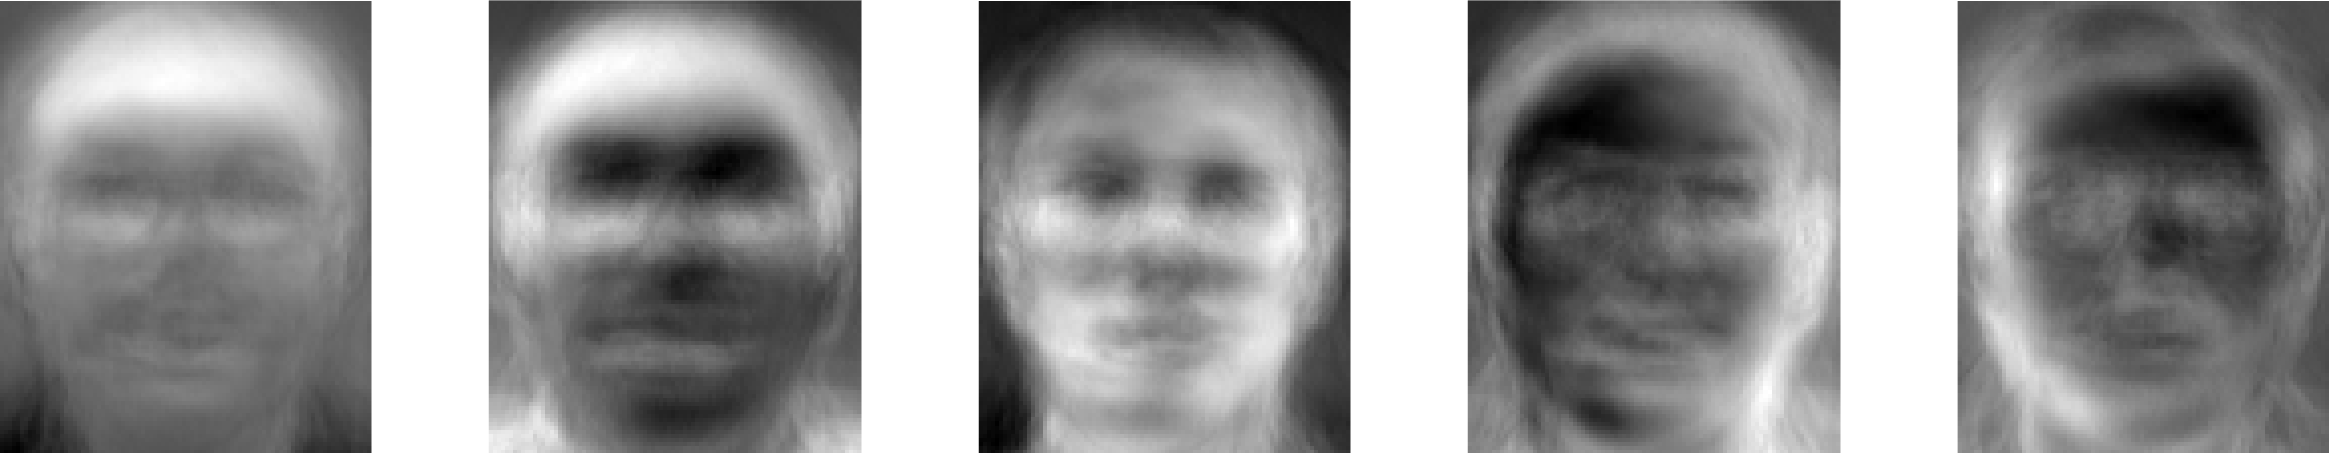
\includegraphics[width=15cm]{5faces}
    \caption{First 5 Eigenfaces}
    \label{5faces}
\end{figure}


\subsection{How does the importance of eigenfaces decrease?}\label{Q1.2}

The first 50 eigenfaces out of 10,304 were found to be of very high importance since it represented 81.61\% of the total variance in the 400 input images as shown in Figure \ref{cum_percents}. Adding more eigenfaces increase the overall importance (variance) but at a slow rate compared to the first 50 i.e. the importance of each eigenface starts decreasing. For instance, the first 100 eigenfaces represent 89.06\% of the total variance, i.e. the second set of 50 eigenfaces account for just around 7.4\% importance compared to 81.61\% by the first 50. 

The importance of each eigenface becomes less further and does not contribute much to the total importance as more eigenfaces are added. The first 400 eigenfaces represents 99.42\% of the total variance. So, addition of more eigenfaces after 400 has nearly no contribution to the total variance. Therefore, the importance of an eigenface decreases almost quadratically up to 400 and then nearly stays constant at 0 up to 10,304 as shown in Figure \ref{cum_percents2}.


\begin{figure}[htp]
    \centering
    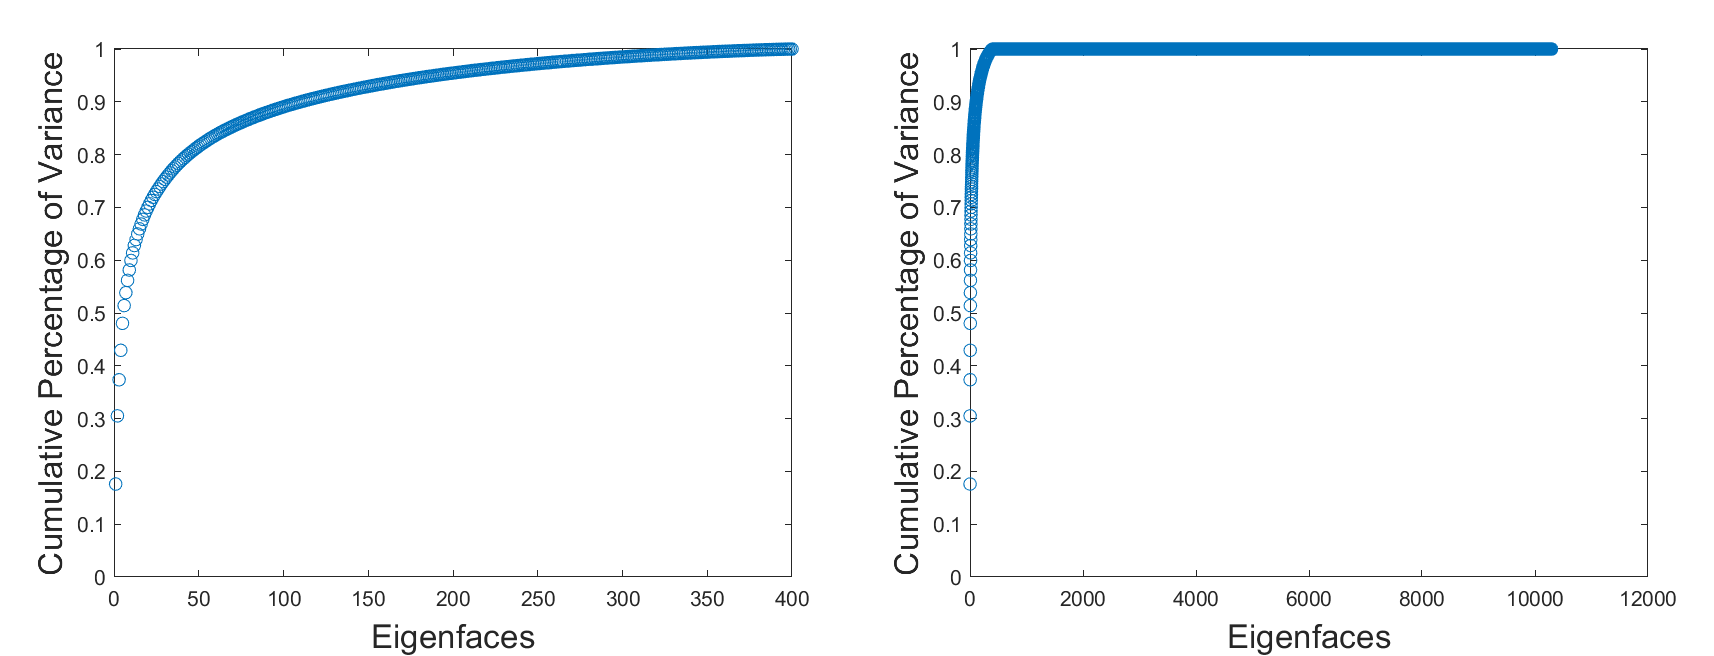
\includegraphics[width=14cm]{cum_percents.png}
    \caption{Eigenfaces and the Cumulative Percentage of Variances Captured. Ranging from 1 to 400 on the left and 1 to 10,304 on the right.}
    \label{cum_percents}
\end{figure}

\begin{figure}[htp]
    \centering
    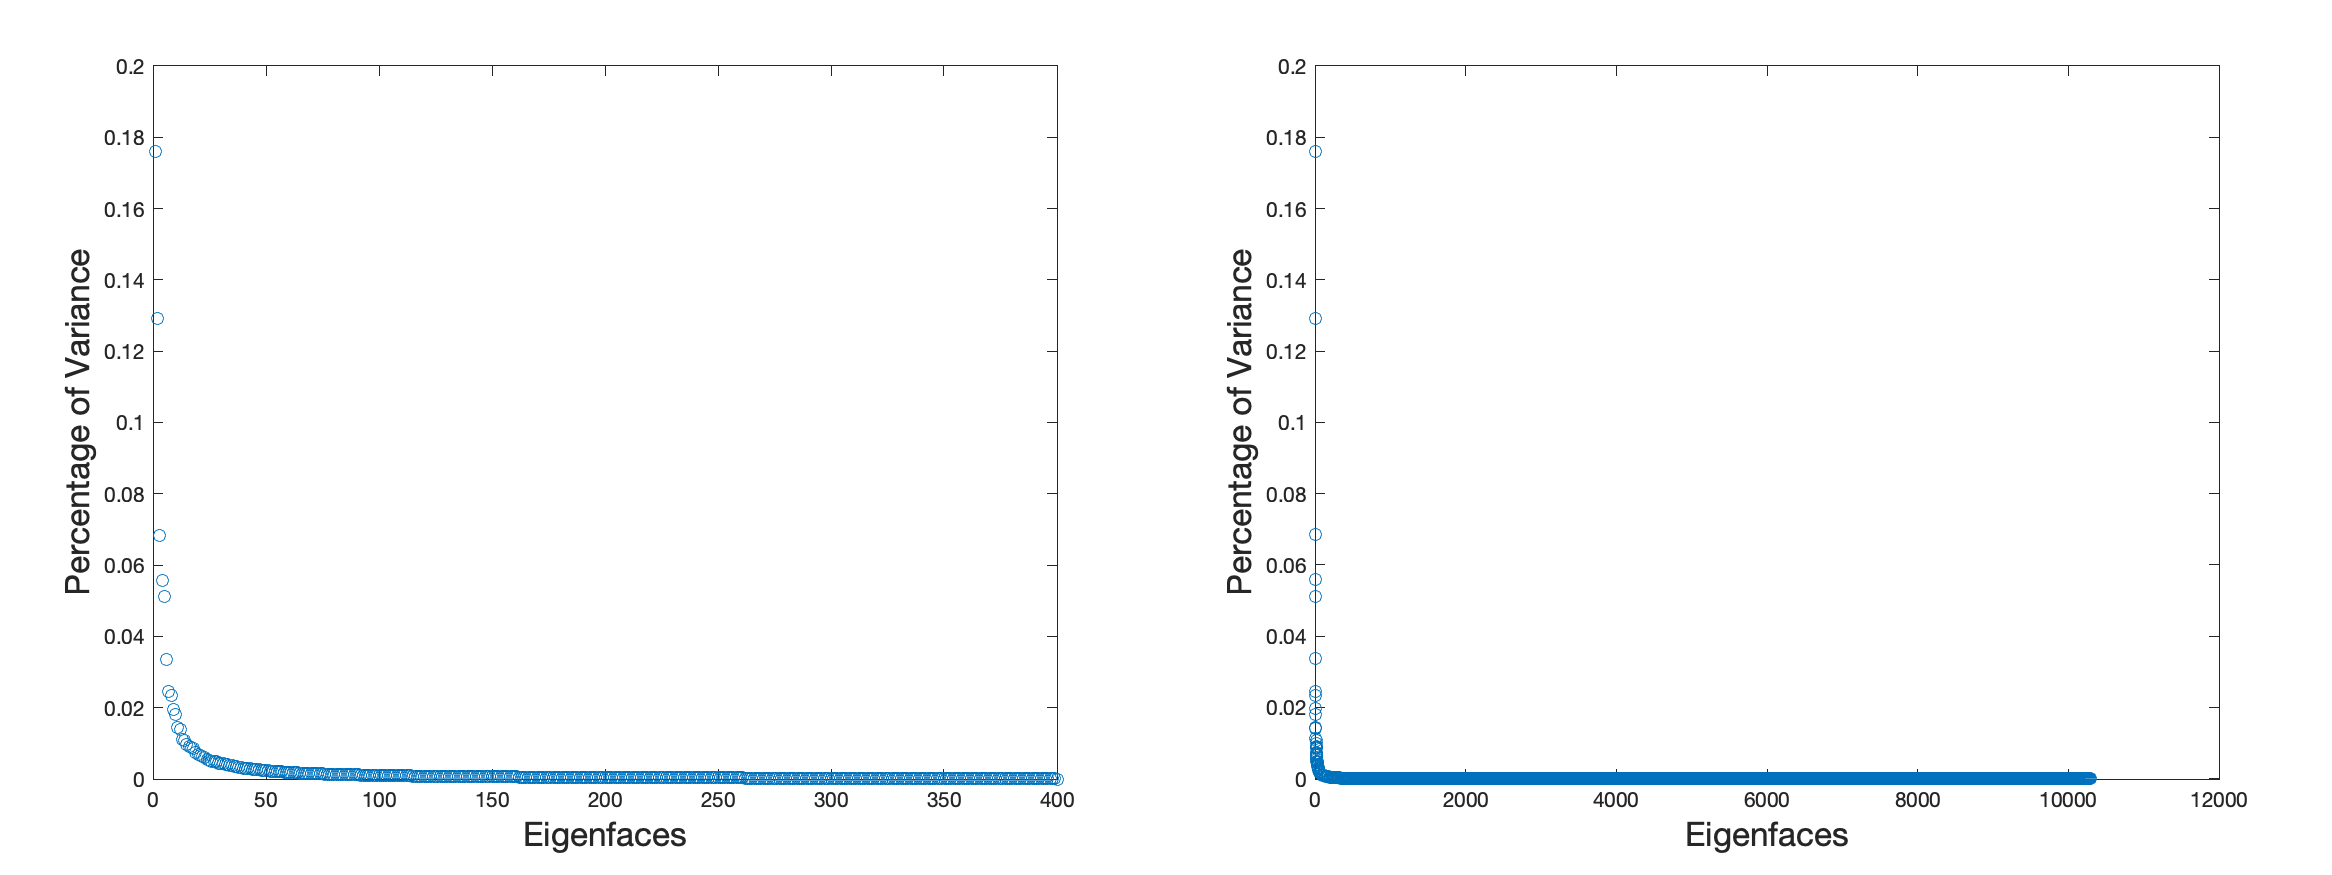
\includegraphics[width=15cm]{graphs2.png}
    \caption{Eigenfaces and the Percentage of Variances Captured. Ranging from 1 to 400 on the left and 1 to 10,304 on the right.}
    \label{cum_percents2}
\end{figure}

\section{Facial Image Reconstruction with PCA}\label{Q2}


\subsection{What is the difference between reconstructed and original images as the number of eigenfaces used in reconstruction increases?}\label{Q2.1}

As the number of eigenfaces used in facial image reconstruction increases, the quality of the reconstructed image increases as well. Using a low number of eigenfaces results in a poor quality and somewhat ``ghostly" reconstructed facial image as in Figure \ref{faces50}  (Turk \& Pentland, 1991). Using a high number of eigenfaces alternatively produces a reconstructed facial image which is almost parallel to that of its original inputted images, such as those shown in Figure \ref{faces400}. This is because those made from the highest number of eigenfaces account for the most variance between the inputted images (See Figure \ref{cum_percents}).  This is the case when using 400 eigenfaces as this was found to capture 99.99\% of the variance of the inputted images. 




\begin{figure}[htp]
    \centering
    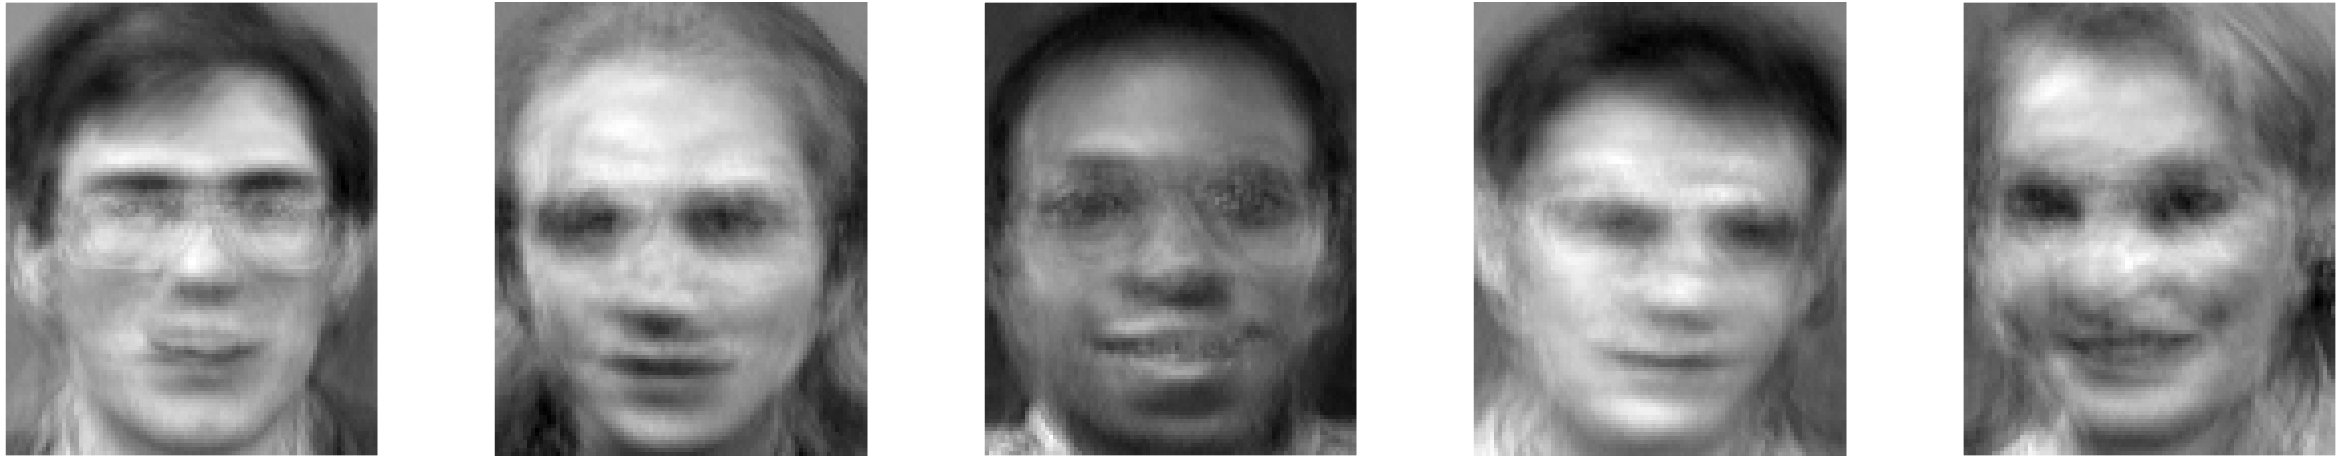
\includegraphics[width=15cm]{faces50.png}
    \caption{Reconstructed Facial Images using 50 Eigenfaces}
    \label{faces50}
\end{figure}

\begin{figure}[htp]
    \centering
    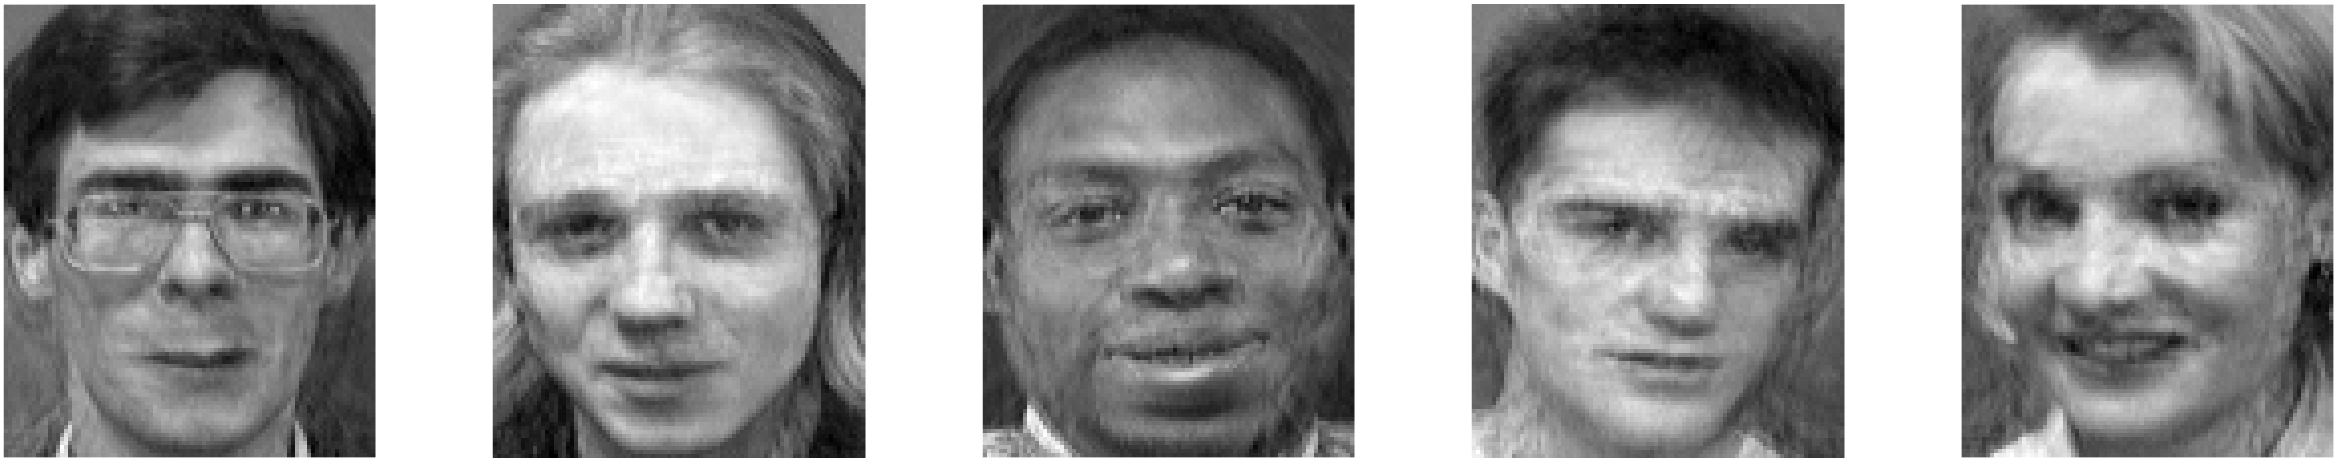
\includegraphics[width=15cm]{faces200.png}
    \caption{Reconstructed Facial Images using 200 Eigenfaces}
    \label{faces200}
\end{figure}

\begin{figure}[htp]
    \centering
    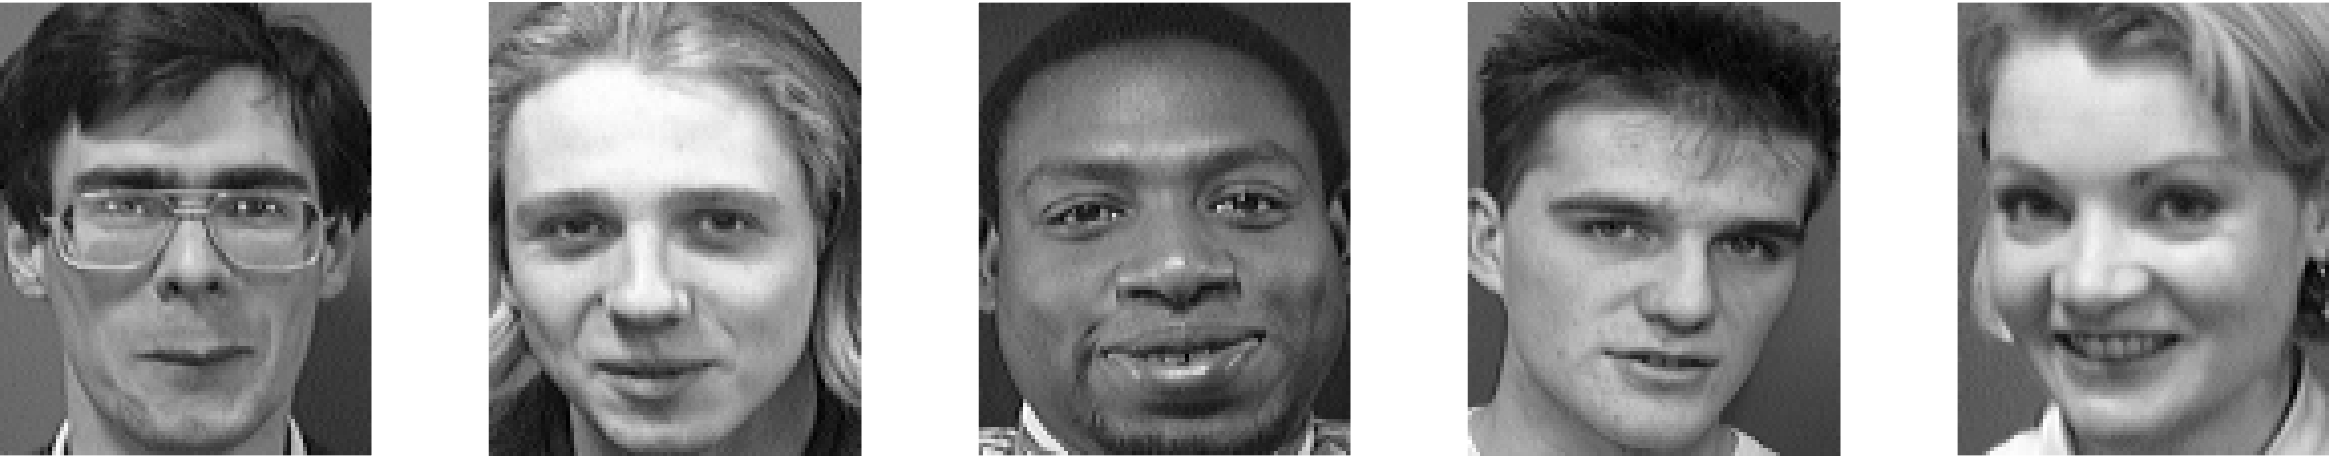
\includegraphics[width=15cm]{faces400.png}
    \caption{Reconstructed Facial Images using 400 Eigenfaces}
    \label{faces400}
\end{figure}




\subsection{How many eigenfaces are required to recover an original face with reasonable errors?}\label{Q2.2}

We defined reasonable error through the use of both the metric Mean Squared Error (MSE) and by comparing visual differences between the original and reconstructed facial images. We found that reconstructed images consisting of 350 eigenfaces generated good quality images with identifiable facial characteristics. These images also had a MSE of 11.073. As a result, we concluded that any reconstructed facial image made from at least 350 eigenfaces and with an MSE value equal to or below 11.073, should be of a good enough quality so as to resemble their inputted original face with reasonable error. 

\begin{figure}[htp]
    \centering
    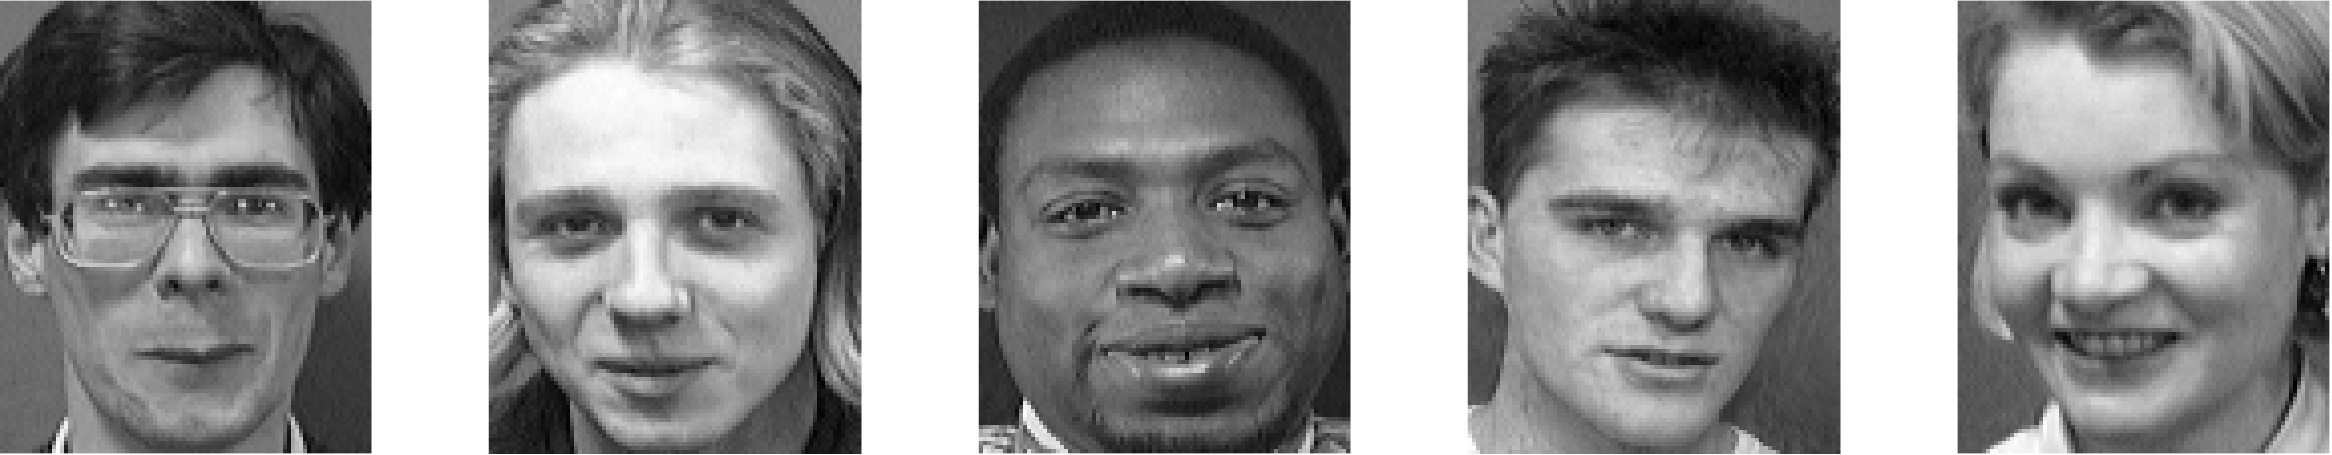
\includegraphics[width=15cm]{faces350.png}
    \caption{Reconstructed Facial Images using 350 Eigenfaces}
    \label{faces350}
\end{figure}

\section{Conclusion}\label{conclusion}
Thus, using PCA, we were able to reduce the dimensions of images from 10,304 to 350 with a very low reconstruction error. Moreover, using 400 dimensions has almost 0 reconstruction error. The ratio of reduction in size is great for various applications. Also, visualizing the eigenfaces as images helped us understand what it represents. For instance, the leading eigenfaces display fundamental facial features like chin,  mouth, nose, ears, hair, etc and all the images are the linear combination of these eigenfaces.




\end{document}